\documentclass[11pt]{article}
\usepackage[utf8]{inputenc}
\usepackage[margin=1in]{geometry}
\usepackage{natbib}
\bibliographystyle{abbrvnat}
\usepackage{amsmath}
\usepackage{amssymb}
\usepackage{comment}
\usepackage{bbm}
\usepackage{amsthm}
\geometry{a4paper}
\usepackage{graphicx}
\usepackage{booktabs}
\usepackage{array}
\usepackage{paralist}
\usepackage{verbatim}
\usepackage{subfig}
\usepackage{multirow}
\usepackage{rotating}
\usepackage{fancyhdr}
\usepackage{hyperref}
\usepackage{bm}
\usepackage{xcolor}
\usepackage{listings}
\lstset{basicstyle=\ttfamily,
  showstringspaces=false,
  commentstyle=\color{red},
  keywordstyle=\color{blue}
}
\pagestyle{fancy}
\renewcommand{\headrulewidth}{0pt}
\lhead{}\chead{}\rhead{}
\lfoot{}\cfoot{\thepage}\rfoot{}
\usepackage{algorithm}
\usepackage{algpseudocode}
\usepackage{fancyvrb}
\usepackage{pythonhighlight}

\title{%
  Data Science - Coursework 2 \\
  \large Comparison of two methods for calculating \\ SHAP values for categorical variables.}
\date{May 2024}
\author{02344391}


\begin{document}

\maketitle
\section*{Introduction}
It is often necessary to explain the predictions made by a machine learning model in order to 
understand the model's decisions. The simplest models, such as linear regression models, can 
be explained by their coefficients. On the other hand, more complex models sometimes require 
the use of an explanatory model to locally explain the predictions associated with each input.

The \href{https://github.com/shap/shap}{SHAP} \textit{Python} module uses Shapley values from 
game theory to explain the predictions of a wide range of models.
According to \cite{lundberg2019consistent}, the module calculates the contribution $\phi_i$ for each 
feature $i$ given an input $u$ on a model $f$ by:

\begin{equation}
    \phi_i = \sum_{S \subseteq N \backslash \{i\}}\frac{|S|!(M-|S| - 1)!}{M !}[f_u(S\cup \{i\})-f_u(S)]
    \label{eq:shap}
\end{equation}

where $N$ is the feature set, $M = |N|$ and:
$$f_u(S) = \mathbb{E}[f(u)|u_S]$$
is the expected value of the function given a subset $S$ of the features of $u$.

In the case of tree-based or ensemble models such as random forest, the \texttt{TreeExpalainer}
class of \href{https://github.com/shap/shap}{SHAP} calculates the Shapley values of each feature 
in an input from the fitted trees. The algorithm calculates $f_u(S)$ in (\ref{eq:shap}) by 
traversing the branches of the decision tree according to the feature values of $S$. When a 
node of the tree corresponds to a feature not included in $S$, the algorithm descends both 
branches under this node. Each of these descents leads to a value. The contribution of the subgroup
$S$ is then the weighted sum of the values obtained by traversing the tree. The weighting corresponds 
to the proportion of samples that passed through the branches of the tree during training.

So we have a method to calculate the contribution of each variable in this kind of models. In this report, 
we will not investigate the consistency of this method for explaining predictions, 
but we will study the particular case where a model has categorical variables that have been 
encoded by One-Hot Encoding. In this case, Shapley values are associated with each of the encoded 
variables. One method to calculate the contribution of categorical variables as a whole is to sum 
the Shapley values of the encoded variables corresponding to the categorical variable. This method for 
calculating the Shapley values of a decision tree assumes that the sub-variables produced by encoding a 
categorical variable are independent. This assumption is inherently false: the encoded sub-variables should 
be considered as a whole when calculating the Shap values using the fitted trees.

The goal of this project is to modify the algorithm calculating the SHAP values of \\ \texttt{TreeExplainer} to consider 
the entire set of sub-variables of a categorical variable as known when it is part of $S$.

\section*{A simple example of a regression tree}

We illustrate the calculation of SHAP values for a short regression tree with a dataset containing a 
numerical variable $x$ and a categorical variable that has been encoded with one-hot encoding $\text{cat}_1$ and $\text{cat}_2$.
We plot in figure (\ref{fig:tree0}) the fitted tree. For the following, we want to analyse the prediction of the input 
$u = (u_x, u_{\text{cat}_1}, u_{\text{cat}_2}) = (60,0,1)$.

\begin{figure}[H]
    \centering
    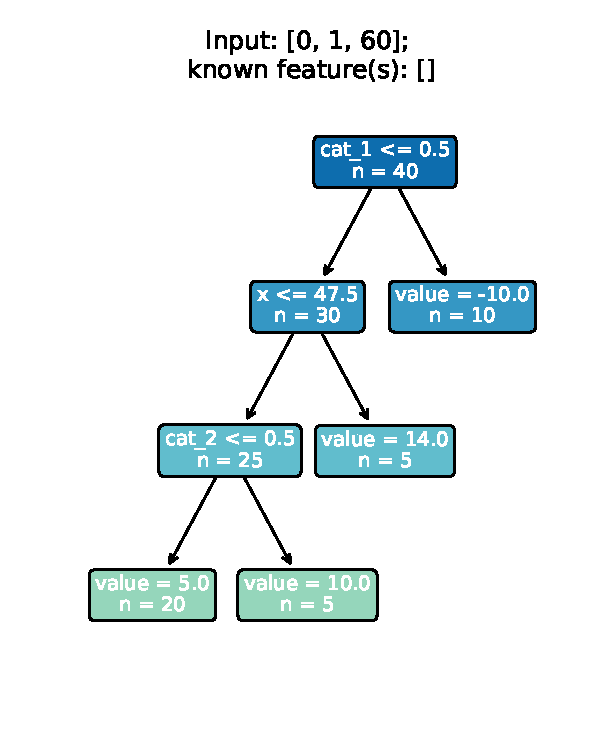
\includegraphics[height=9cm]{"../outputs/plot_tree/figures/path_0_known.pdf"}
    \caption{Plot of the fitted tree. The colored nodes correspond to the paths taken 
    by the algorithm when certain features of an input are known. Here, we consider that 
    no feature is known.}
    \label{fig:tree0}
\end{figure}

In figure (\ref{fig:tree0}), we consider that no feature is known, which corresponds to 
$$f_u(S) = f_u(\{\}) = \mathbb{E}[f(X)] = \frac{1}{40}\left(20 \times 5 + 5 \times 10 + 5 \times 14 + 10 \times (-10)\right)$$

the mean value of the prediction on the training set.

In figure (\ref{fig:tree1}), we plot the tree paths when one feature is known: $S = \{x\}$ or $S = \{\text{cat}_1 \}$ or $S = \{\text{cat}_2 \}$.
We find that 
\begin{align*}
    & f_u(\{\text{cat}_1 \}) = \frac{22}{3}\\
    & f_u(\{\text{cat}_2 \}) = \frac{11}{2}\\
    & f_u(\{ x \}) = 8
\end{align*}

\begin{figure}[H]
    \centering
    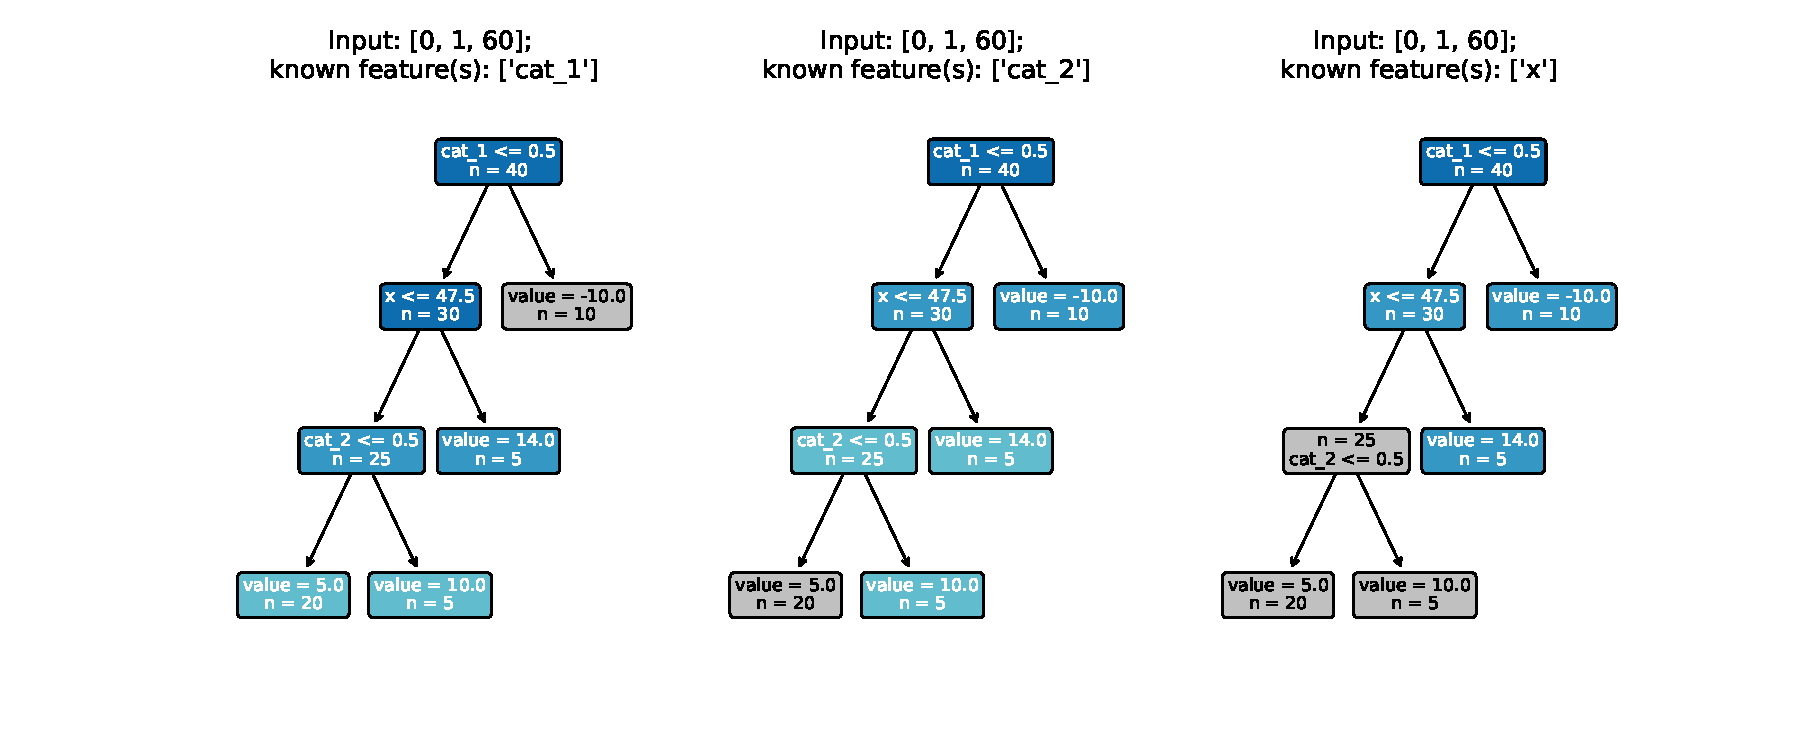
\includegraphics[height=6.6cm]{"../outputs/plot_tree/figures/path_1_known.pdf"}
    \caption{Plot of the fitted tree. The colored nodes correspond to the paths taken 
    by the algorithm when certain features of an input are known. Here, we consider that 
    one feature is known.}
    \label{fig:tree1}
\end{figure}

In figure (\ref{fig:tree2}), we plot the tree paths when two features are known: $S = \{\text{cat}_1, \text{cat}_2\}$ or $S = \{\text{cat}_2, x \}$ or $S = \{\text{cat}_1, x \}$.
We find that 
\begin{align*}
    & f_u(\{\text{cat}_1, \text{cat}_2\}) = \frac{32}{3}\\
    & f_u(\{\text{cat}_2, x \}) = 8\\
    & f_u(\{\text{cat}_1, x\}) = 14
\end{align*}

\begin{figure}[H]
    \centering
    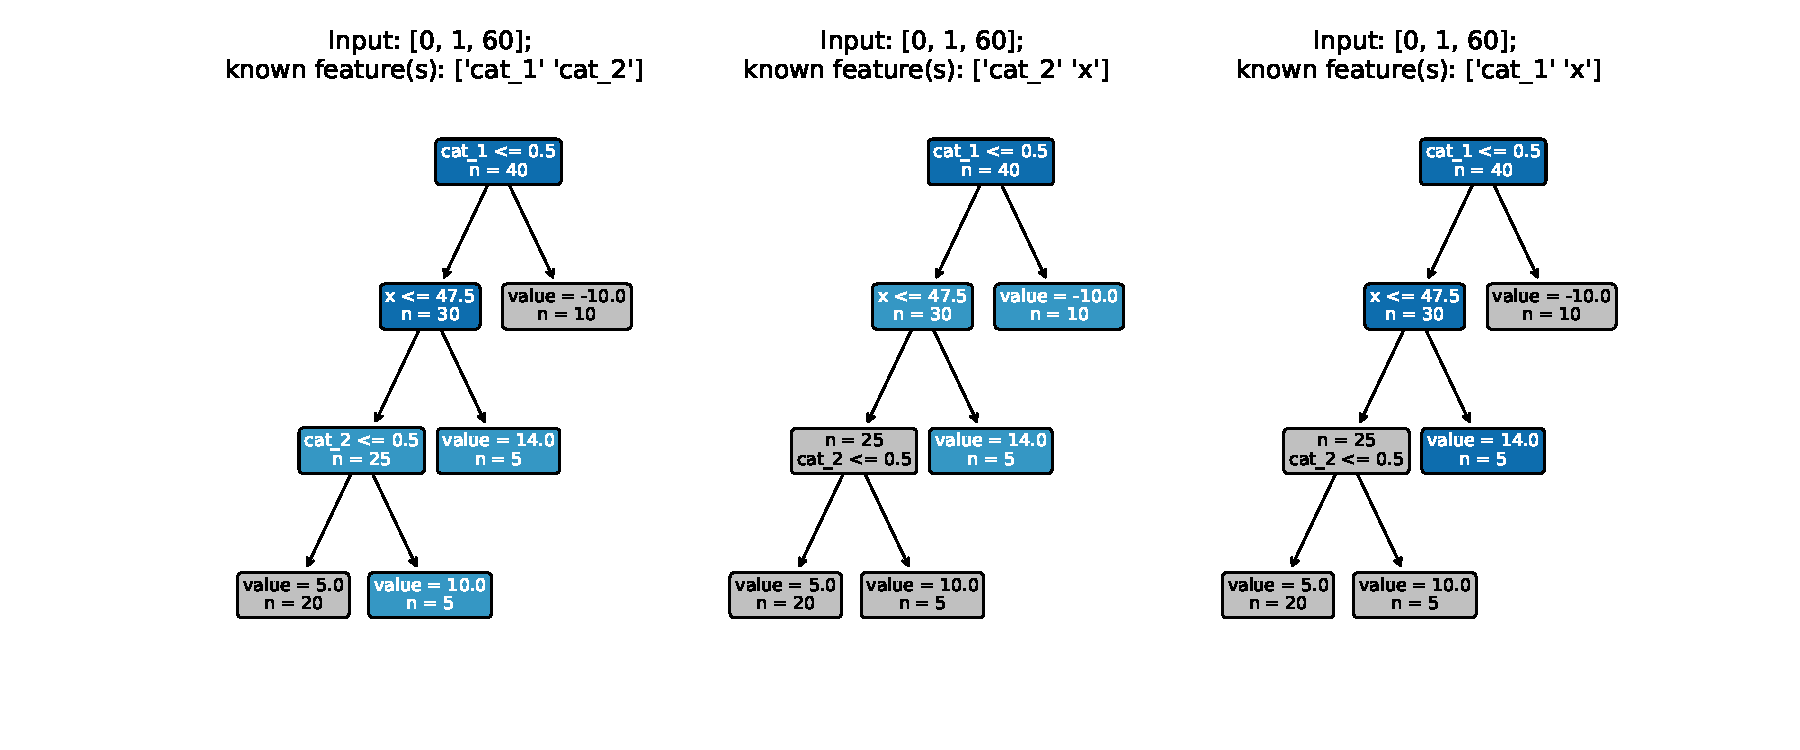
\includegraphics[height=6.6cm]{"../outputs/plot_tree/figures/path_2_known.pdf"}
    \caption{Plot of the fitted tree. The colored nodes correspond to the paths taken 
    by the algorithm when certain features of an input are known. Here, we consider that 
    two features are known.}
    \label{fig:tree2}
\end{figure}


Finally, we plot in figure (\ref{fig:tree3}) the tree paths when all the features are known: 
$$S = \{\text{cat}_1, \text{cat}_2, x\}.$$
We find that 
$$f_u(\{\text{cat}_1, \text{cat}_2, x\}) = 14$$


\begin{figure}[H]
    \centering
    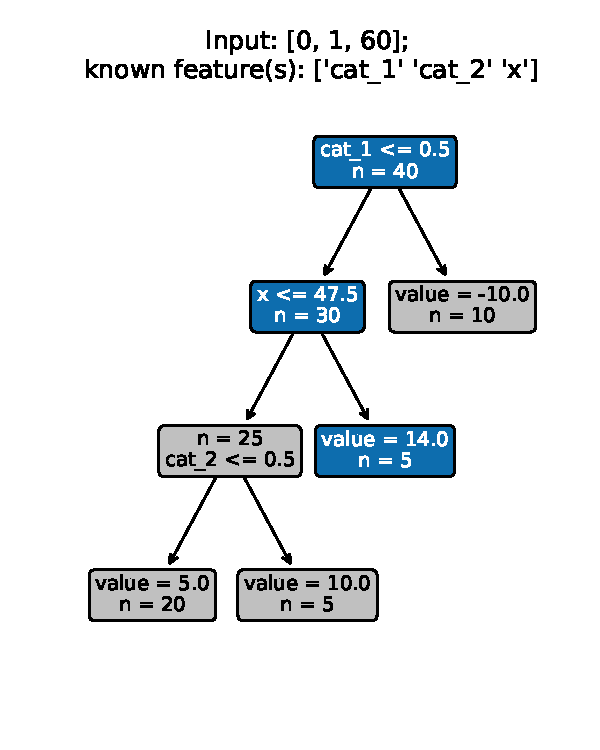
\includegraphics[height=9cm]{"../outputs/plot_tree/figures/path_3_known.pdf"}
    \caption{Plot of the fitted tree. The colored nodes correspond to the paths taken 
    by the algorithm when certain features of an input are known. Here, we consider that 
    three features are known.}
    \label{fig:tree3}
\end{figure}

By applying formula \ref{eq:shap} to each of the features, we obtain:
\begin{align*}
    & \phi_x = \frac{155}{36} \approx 4.3056\\
    & \phi_{\text{cat}_1} = \frac{191}{36} \approx 5.3056 \\
    & \phi_{\text{cat}_2} = \frac{25}{18} \approx 1.3889
\end{align*}

And on the other hand, if we redo the calculation considering that $\text{cat}_1$ and $\text{cat}_2$ form 
a set cat of cardinality 1 and are inseparable, the SHAP values become:
\begin{align*}
    & \phi_x' = \frac{25}{6} \approx 4.1667\\
    & \phi_{\text{cat}} = \frac{41}{6} \approx 6.8334
\end{align*}

We observe that $\phi_{\text{cat}} \neq  \phi_{\text{cat}_1}+\phi_{\text{cat}_2} $ and 
$\phi_x \neq  \phi_x'$. However, the values are quite close. Next, we will 
compare these two methods for different datasets to see if they lead to similar results.

\newpage
\bibliography{bibliography}
\end{document}